\chapter{Measurements of extreme first passage times in photon transport}


\begin{abstract}
    Photon transport through turbid media has typically been modeled through diffusion or telegraph equations. These models describe behavior of the average, or typical, photon with remarkable accuracy, however, we show here that they fail to capture the Extreme First Passage Times (EFPTs) of photon transport. By sending ultra-fast bursts of photons through a scattering medium and timing the arrival of the first passage photon, we measure the distribution of these EFPTs of photons in a random environment. Our measured EFPTs differ from those predicted by both the diffusion approximation and telegraph equation. Instead, we observe the EFPT as the time expected for light to travel through an index-averaged medium. These results reveal flaws in both models and invite a re-examining of their underlying assumptions.
\end{abstract}




\acg{[note: Optics Letters has no section titles]}
\section{Introduction}

When light passes through a scattering medium, the spatial distribution of photons is smeared out by random scattering events, resulting in a corresponding broadening of the distribution of photons from a pulsed source. This broadening has historically been modeled at short times by the telegraph equation~\cite{goldstein_diffusion_1951,ishimaru_diffusion_1989,durian_photon_1997,lemieux_diffusing-light_1998} and at asymptotically long times by the diffusion approximation~\cite{haskell_boundary_1994,bohren_absorption_1983,ishimaru_wave_1997}.  However, these models both rely on a central assumption, that the scattering, and thus the path through the system, of each photon is independent and identically distributed.  Here, we probe the quality of these models by examining a measurement of the Extreme First Passage Time (EFPT), that is, the \textit{first} time of first arrival within a pulse of light.  We use a femtosecond laser to fire pulses of light through a tunable scattering medium and measure the EFPT with a Single Photon Avalanche Diode (SPAD).  We present experimental evidence that both of these models provide quantitatively and qualitatively wrong predictions for this measurement. 


\acg{[Optica papers require a short summary paragraph.] 
In this Letter, we describe work to date on describing photon first passage distribution, then describe an experimental setup that allows us to measure photon EFPT. We describe the diffusion approximation and telegraph equation approaches to modelling photon transport, and compare EFPT predictions from these models to experimental measurements. We demonstrate that both models fail to predict the EFPT.}

\section{Background}

Two widely used approximations for modeling photon transport are the diffusion approximation and the telegraph equation. The diffusion approximation predicts the bulk or average behavior of light pulses in random media and offers valuable insights into various systems across a broad range of applications~\cite{haskell_boundary_1994, chandrasekhar_radiative_1950,  brown_light_1975, chandrasekhar_stochastic_1943, allgaier_diffuse_2021, taitelbaum_diagnosis_1999, amendola_accuracy_2021}. However, the diffusion approximation neglects ballistic photons by disregarding the speed of light, making it unsuitable for: short length and time scales, \acg{\st{scenarios} media} with significant anisotropy or absorption, and environments with low scattering~\cite{ishimaru_wave_1997, yoo_time-resolved_1990, yoo_when_1990, durian_photon_1997, zhang_wave_2002, pierrat_photon_2006}. The telegraph equation overcomes many of these limitations by accounting for the finite speed of light in a medium and capturing wave-like effects at small distances, providing a more accurate description of the bulk or typical behavior of light pulses~\cite{goldstein_diffusion_1951, durian_two-stream_1996, durian_photon_1997, lemieux_diffusing-light_1998, masoliver_solutions_1992, masoliver_finite-velocity_1996, das_non-fickian_1998, polishchuk_photon-density_1997}. Discrepancies remain at distances near the source relative to the transport mean free path~\cite{durian_photon_1997, dudko_photon_2005, lemieux_diffusing-light_1998}, and the accuracy of the predicted speed of light depends on how the scattering path length and anisotropy are treated during the derivation~\cite{ heizler_asymptotic_2012, hoenders_telegraphers_2005, polishchuk_photon-density_1997}.

First passage times have been broadly described and studied across various diffusive systems~\cite{redner_8_2001,weiss_applications_2002,godec_first_2016,noskowicz_average_1988}, including chemical and molecular reactions~\cite{redner_8_2001,grebenkov_molecular_2021}, protein interactions~\cite{polizzi_mean_2016}, fractal media~\cite{chun_heterogeneous_2023}, and stock market fluctuations~\cite{barney_first-passage-time_2017,zsurkis_first_2024}. In general, extreme value distributions, which describe values drawn from the tails of a source distribution, exhibit distinct statistical behaviors~\cite{lawley_distribution_2020,lawley_universal_2020} and play a critical role in processes such as menopause timing~\cite{lawley_slowest_2023}, gene activation~\cite{schuss_redundancy_2019}, and oocyte fertilization by sperm~\cite{meerson_mortality_2015,schuss_redundancy_2019}.  In photonic systems, changes in pulse shape due to absorption and scattering have been measured~\cite{lee_using_2007,madsen_experimental_1992,ishimaru_diffusion_1978,yoo_time-resolved_1990,yoo_when_1990,zhang_wave_2002,calba_ultrashort_2008}, and photon FPT distributions have been characterized numerically and experimentally~\cite{rossetto_isotropic_2022,long_particle_2001,weiss_applications_2002,zeller_light_2020}. \acg{To our knowledge, EFPT distributions have not been measured experimentally.}

\begin{figure}[htp]
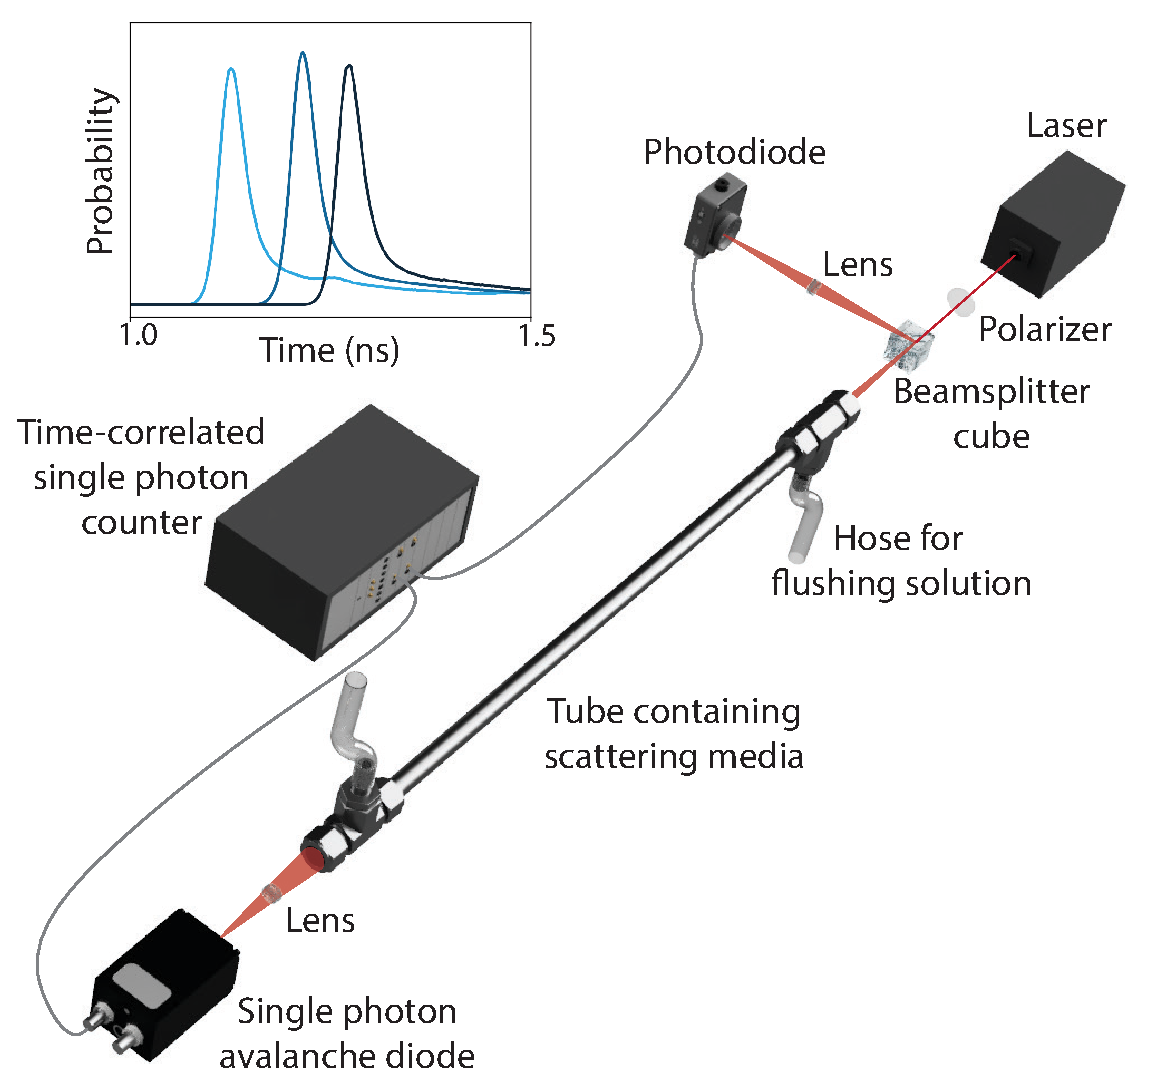
\includegraphics[width=0.8\columnwidth]{Figures/exp-setup-3.pdf}
\caption{\label{fig:setup}  Experimental setup, consisting of elements described in the text. The signals are collected over an adjustable time period, resulting in a histogram of EFPTs. An example of such a histogram at three different concentrations of scattering media is shown, with concentration increasing from left to right, where the x axis is the time relative to the speed of light in a vacuum, and the y axis is the probability of that time as the EFPT.}
\end{figure}

\section{Experimental Methods}\label{sec:exp_meth}

Our experimental setup is shown in Figure \ref{fig:setup}. Optical pulses of 140 fs in duration are generated with a femtosecond pulsed laser (Coherent Chameleon Ultra II laser) operating at central wavelengths tunable between 680-1080 nm with a repetition rate of 80 MHz and wavelength-dependent total output power range of 650-3500 mW. These pulses are sent through a power attenuating polarizer (Thorlabs GL10-B).  The majority of the power is bled off through a beamsplitter (Thorlabs BS041) and sent to a photodiode (Thorlabs DET10A).  This photodiode triggers a time-correlated single photon counter (TCSPC) (PicoQuant HydraHarp 400) to start a time-of-flight measurement.  The majority of the light continues into a 12.7mm diameter, 1.015 m long stainless steel tube that has been internally polished.  This tube is filled with a solution of water and 20 nm diameter silica nanospheres (LUDOX AS-40) with index of refraction $n$ = \acg{1.453-1.456, dependent on wavelength}.  The concentration of nanospheres is \acg{variable}, in place, from volume fractions of 0 to 0.235 parts silica to 1 part water, \acg{where the maximum value} is the volume fraction of undiluted LUDOX. \acg{The medium is changed by} flushing the solution and flowing in a new solution.  After traveling through the scattering medium, photons exit the tube and are concentrated through a doublet lens (Thorlabs AC254-030-B-ML) onto a Single Photon Avalanche Diode (Micro Photon Devices PDM series SPAD).  The signal from the SPAD triggers the TCSPC to stop and the time of flight measurement is recorded. 

The  TCSPC and SPAD both have a dead-time less than 80 ns, yielding an effective experimental repetition rate of 12.5 MHz. Using a detector for the TCSPC start and stop signals allows for measurement resolution that is not limited by the dead time. Integration times varied from 1-600 s.

\acg{The SPAD detection efficiency varies with wavelength from 10-30\%. From the peak laser power, approximately 3.5 W at 750 nm light, repetition rate of 80 MHz, and power attenuation from the optical components, we find a generous upper bound for the number of photons per pulse, $N$, entering the system as $5 \times 10^{6}$.}

We use Ludox AS-40 as a scattering medium because it scatters strongly, absorbs minimally, is easily diluted with water, and the silica does not aggregate \acg{[is it worth saying that sonicating can break up aggregates? I sonicated some solutions that had clearly aggregated and EFPT results were exactly the same]}. Ludox has also been well characterized for light scattering purposes~\cite{dezelic_determination_1960,bonnelycke_light_1959,goring_light-scattering_1957}. The small size of the silica nanospheres (roughly 3\% of the wavelengths used in these experiments) places us firmly within the Rayleigh scattering regime for which we can calculate $\sigma_{s}$ and $\mu_{s}$, the scattering cross section and coefficient, as~\cite{bohren_absorption_1983, chandrasekhar_radiative_1950} 
%
\begin{equation}\label{eq:scatter}
    \sigma_{s} =  \frac{2 \pi^{5}}{3} \frac{d^{6}}{\lambda^{4}}\left(\frac{n_{silica}^{2}-n_{water}^{2}}{n_{silica}^{2}+2n_{water}^{2}}\right)^{2},\ \mu_{s} = \frac{C}{\frac{4}{3} \pi \left(\frac{d}{2}\right)^{3}} \sigma_{s}
\end{equation}
%
where $d$ represents the scatterer diameter, $\lambda$ is the wavelength of light being scattered, $n$ is the refractive index of the scatterer material, $C$ is the volume concentration of scatterers, and the scattering coefficient is the inverse of the scattering path length with units $\frac{1}{\textrm{m}}$. Using measurements performed with a UV/Vis/NIR spectrophotometer (Perkin Elmer Lambda-1050), we further characterize this medium by measuring $\sigma_{a}$, the absorption cross section \acg{[technically I measure absorptivity and then calculate cross section?]}, and use the Beer-Lambert law to find $\mu_{a}$, the absorption coefficient, as~\cite{lakowicz_principles_2006} 
%
\begin{equation}\label{eq:absorb}
    \sigma_{a} = 1.53\times 10^{-22}\ \textrm{m}^{2},\ \mu_{a} = \frac{C}{\frac{4}{3} \pi \left(\frac{d}{2}\right)^{3}} \sigma_{a}.
\end{equation}
%
\acg{[NOTE: if useful to include, here lies the exact way to get from measured molar attenuation (in this case absorption) coefficient $\epsilon = 0.04$ to the absorption cross section $\sigma_{a}$}
%
\begin{equation}
    \acg{\sigma_{a} = \ln{10} \frac{\rho_{water}}{N_{A}} \frac{\log_{10}\left(\frac{I_{0}}{I}\right)}{l C} }
\end{equation}
\acg{where $l$ is the path length of the cuvette, $C$ is the concentration of the solution, $I$ is the light intensity emitted, $I_{0}$ is the light intensity detected, $N_{A}$ is Avogadro's number, and $\rho_{water}$ is the density of water.}]
%
\section{Models for Photon Transport}\label{sec:predictions}
A common approach for modeling photon transport is to start with the equation of transfer\acg{. As there is currently no general solution to the time-dependent radiative transfer equation, most applications rely on} approximations to derive a more tractable solution. Different \acg{approximation methods} yield distinct solutions, with the diffusion approximation and the telegraph equation being two widely used outcomes. In the following, we approximate the transmission of light through a slender tube filled with scattering medium as a one-dimensional process. We describe these two approaches below, resulting in two distinct photon probability distributions. From the probability distribution of photon locations, we derive an approximation for the extreme first passage time (EFPT) past a distance $L$. We approximate this as the first time at which the cumulative probability beyond $L$ surpasses 1/$N$, for $N$ incident photons~\cite{hass_first-passage_2024}. \acg{Thus, for $N$ particles, at this time value we expect at least one photon to be located past $L$.}


\subsection{The equation of transfer}
A classical approximation to the spatial and temporal distribution of photons is the equation of transfer ~\cite{haskell_boundary_1994,ishimaru_wave_1997}.,
%
\begin{align}
    \frac{1}{c} &\partial_{t} L \left(\mathbf{r},\hat{s},t\right) + \mathbf{\nabla} \cdot L\left(\mathbf{r},\hat{s},t\right)\hat{s} = -\left(\mu_{s} + \mu_{a}\right) L\left(\mathbf{r},\hat{s},t\right) \nonumber \\
    &+ \mu_{s} \int \int_{4\pi} L\left(\mathbf{r},\hat{s'},t\right) f\left(\hat{s} \cdot \hat s'\right) d\Omega' + S\left(\mathbf{r},\hat{s},t\right). \label{eq:RTE}
\end{align}
%
This equation determines the rate of change of the radiance, $L$, through position $\mathbf{r}$, in direction $\hat s$, and at time $t$. The radiance originates at a source, described by $S$, and is lost to the absorption coefficient, $\mu_{a}$, and scattered by the scattering coefficient, $\mu_{s}$. The speed of light in the medium is $c$, and $f(\hat s \cdot \hat s')$ is the normalized differential scattering probability for photons travelling in a direction $\hat s'$ to scatter into the direction $\hat s$. 

\eqref{eq:RTE} can be integrated over all solid angles to find a continuity equation governed by the photon density, $\varphi\left(\mathbf{r}, t\right)$, and photon flux, $\mathbf{j}\left(\mathbf{r}, t\right)$~\cite{haskell_boundary_1994}. When considering scattering in a long tube it is useful to approximate the system as quasi-one-dimensional.  Because $f\left(\hat{s}\cdot\hat{s}'\right)$ can be thought of as a distribution of scattering angles where $\cos \theta = \hat s \cdot \hat s'$, it will reduce to a single parameter \acg{\st{$g =$}} $\langle\cos{\theta}\rangle$ when integrated over all angles. For Rayleigh scattering, which is isotropic in both forward and backward directions~\cite{bohren_absorption_1983}, \acg{ $\langle\cos{\theta}\rangle = 0$.}

\subsection{Diffusion approximation}\label{sec:diffusion}

When the total volume concentration of scatterers greatly exceeds 1\%, \eqref{eq:RTE} can be estimated by a diffusion approximation. Under the assumption that photons interact with many particles, we can assume a nearly uniform angular scattering distribution~\cite{ishimaru_wave_1997,bohren_absorption_1983}. By expressing the radiance $L\left(\mathbf{r},t\right)$ as the sum of an isotropic photon density $\varphi\left(\mathbf{r}, t\right)$ and a small directional flux, neglecting variations and anisotropy in the source term $S\left(\mathbf{r},t\right)$, integrating over all solid angles, and approximating as a one-dimensional system, we obtain~\cite{haskell_boundary_1994}
%
\begin{equation}\label{eq:diff}
    D \partial_{r}^{2} \varphi \left(r,t\right) - \mu_{a} c \varphi \left(r,t\right) = \partial_{t} \varphi \left(r,t\right) - c S \left(r,t\right),
\end{equation}
%
with diffusion coefficient
\begin{equation}\label{eq:diffD}
    D = \frac{c}{3\left(\mu_{s} + \mu_{a}\right)},
\end{equation}
$c$  the speed of light in the medium The solution to \eqref{eq:diff} is well-established as a Gaussian multiplied by a decaying exponential term that accounts for absorption~\cite{haskell_boundary_1994}.


Under this diffusion approximation photons move as Brownian walkers in a semi-infinite medium, starting at the origin and whose position we denote as $B(t)$. \acg{\st{Due to absorption, the integrated probability density decays as $\exp{-\mu_{a} t}$.  Thus, one can express} When absorption is minimal,} the probability of a photon to be found beyond a distance $L$ at time $t$ \acg{can be expressed} as~\cite{redner_8_2001,lawley_distribution_2020}
\begin{align}\label{eq:diffProb}
     P\left(B\left(t\right) \geq L\right) = 1-\textrm{erf}\left(\frac{L}{2 \sqrt{D t}}\right).
\end{align}
We approximate the expected value of the EFPT as the time at which this probability surpasses $1/N$. We note that at short times the diffusion approximation yields non-physical behavior \acg{because the photon speed is undefined}.


%%%
%\acg{[A paragraph on Lawley 2020 predictions instead of the previous?]}
%For photons modelled as Brownian walkers in a semi-infinite medium, assuming a large number of photons in each pulse, we can expect the EFPT distribution to be Gumbel, with the shape of the distribution determined by the number of photons $N$, the distance from the origin $L$, and the diffusion coefficient $D$~\cite{lawley_distribution_2020}. We can then determine the expected time $t$ corresponding to the peak of this distribution, and compare this to the measured results.
%%%

\begin{figure}[htp]
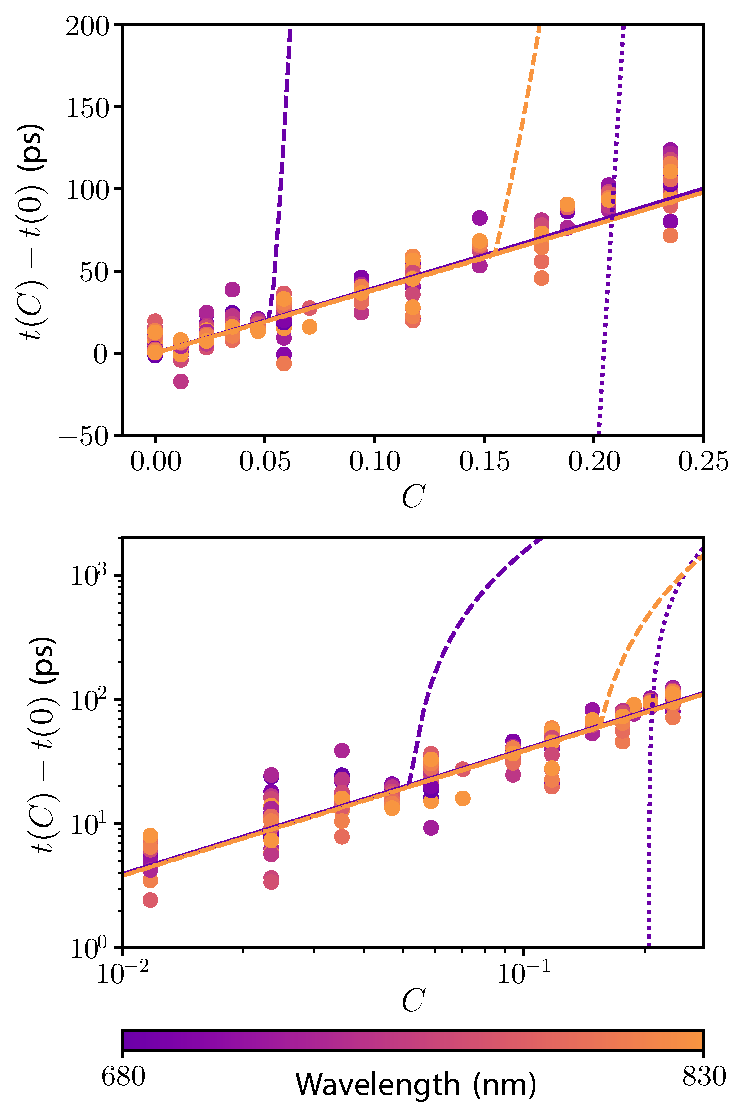
\includegraphics[width=0.75\columnwidth]{Figures/final_predictions_with_data.pdf}
\caption{\label{fig:alldata} FPT differences measured experimentally, in picoseconds, versus volume concentration $C$. The upper and lower plots are the same, with different scales. The solid cyan line is the predicted FPT for a photon traveling through a medium where the index of refraction is averaged for silica and water at that concentration, a value which has negligible variation between these wavelengths. The experimental values are shown as points, the telegraph equation predictions are shown as dashed lines, the diffusion approximation is shown as dotted lines, and color indicates wavelength from 680 nm (violet) to 830 nm (orange). \acg{[If useful, the peak of these distributions is at least $40$ times higher than the noise floor, and the standard error is around 4-12 ps depending on wavelength/power/concentration/etc]}}
\end{figure}

\subsection{Telegraph equation}\label{subsec:teleg} 
The telegraph equation  offers a more accurate model for photon transport, incorporating the ballistic motion of photons. By using asymptotic expansions to approximate a solution to  \eqref{eq:RTE} ~\cite{heizler_asymptotic_2012, hoenders_telegraphers_2005, gombosi_telegraph_1993}, accounting for the movement of photons in and out of each direction as opposing ``streams''~\cite{schuster_radiation_1905,durian_two-stream_1996,lemieux_diffusing-light_1998,masoliver_solutions_1992}, or by various other methods of derivation~\cite{goldstein_diffusion_1951,dudko_photon_2005,masoliver_finite-velocity_1996,weiss_first_1984,weiss_applications_2002}, we arrive at a telegraph equation for photon transport~\cite{lemieux_diffusing-light_1998}, which governs the evolution of $\varphi$ as
\begin{align}
     \partial_{r}^{2} \varphi \left(r,t\right)  = &\frac{1}{c^{2}}\partial^{2}_{t} \varphi\left(r,t\right) + \frac{1}{c}\left(2 \mu_{a} + 3 \mu_{s} \right) \partial_{t} \varphi\left(r,t\right) \nonumber \\
    &+ \mu_{a}\left(\mu_{a} + 3 \mu_{s} \right) \varphi. \label{eq:tel}
\end{align}
At short times, \eqref{eq:tel} reduces to the wave equation. At long times in the limit of $\mu_{a}$ going to zero we recover \eqref{eq:diff}, the standard diffusion approximation, with diffusion coefficient~\cite{lemieux_diffusing-light_1998}
\begin{equation}\label{eq:telD}
    D = \frac{c}{3\mu_{s}}.
\end{equation}

The general solution to this telegraph equation is given by~\cite{goldstein_diffusion_1951,durian_photon_1997}
\begin{align}
    \varphi \left(r,t\right) &= \frac{1}{2} e^{-\left(\mu_{a}c + \gamma \right)t} \bigg[\delta \left(c t - r\right) + \delta\left(ct + r\right) \notag\\
    &+\left. \Theta\left(c t - |r|\right) \left(\frac{\gamma}{c}I_{0}\left(\frac{\gamma u}{c}\right) + \frac{\gamma t}{u}I_{1}\left(\frac{\gamma u}{c}\right)\right)\right]
\end{align}

where $\delta$ is the Dirac delta function, $\Theta$ is the Heaviside step function, $I_{0}$ and $I_{1}$ are the modified Bessel functions of the first kind, $u=\sqrt{c^{2}t^{2}-r^{2}}$ represents the position relative to the maximum photon distance, and $\gamma = \frac{3}{2} c \mu_{s}$ is a characteristic time scale for scattering events~\cite{goldstein_diffusion_1951,masoliver_solution_1993,masoliver_telegraphers_1994,masoliver_finite-velocity_1996}. We solve this numerically to obtain EFPT predictions.

\section{Results and Discussion}

Figure \ref{fig:alldata} shows $t(C)$, the time of the peak of the EFPT distribution for scatterer volume concentration $C$, for a range of wavelengths and volume concentrations. For each wavelength measured, this time is shown relative to $t(0)$, the time of the peak of the EFPT distribution for pure water recorded at that wavelength. The measured EFPTs show no wavelength dependence and increase linearly with $C$, reaching \acg{approximately 100} ps for $C$ = 0.235. The measured EFPT differences are consistent with the extreme photons traveling at the speed of light through a \textit{non-scattering} index-averaged medium at each concentration. \acg{Note that because these measurements are independent of wavelength, and the wavelength-dependent properties $\mu_{a}$ and $\mu_{s}$ significantly impact bulk photon dynamics and mean arrival time but do not affect the EFPT. Additionally, despite expectations that lower $N$ would increase EFPT, the values for $N$ ranged from approximately $10^{3}$ to $10^{6}$ from the wavelength-dependent power output, and this variation did not affect the measured data.}

The predictions of the two models are plotted as dotted lines (diffusion approximation) and dashed lines (telegraph equation) for wavelengths at the extreme ends of our experimental range. These predictions are calculated using $N \simeq 5 \times 10^{6}$. \acg{Because t}he EFPT increases with decreasing $N$~\cite{lawley_distribution_2020}, this \acg{upper limit for $N$} gives us a lower bound on the predicted values of the peak EFPT, \acg{since smaller values for $N$ would produce even larger delays in EFPT. Additionally, the difference between the predictions at 680 nm and 830 nm becomes larger as $N$ decreases.} The diffusion approximation predicts non-physical results for lower concentrations, allowing photons to travel faster than the speed of light for $C$ below approximately \acg{0.21 at 680 nm, and for all concentrations at 830 nm}. At higher concentrations, the diffusion approximation predicts increasing EFPT differences, exceeding \acg{650 ps (680 nm) at $C$ = 0.235}.  The telegraph equation, in contrast, predicts a linear relationship for EFPT delay at low concentrations, determined by the speed of light in the index-averaged medium. However, for concentrations beyond approximately \acg{0.05 (680 nm) and 0.15 (830 nm)}, scattering and absorption cause the EFPT difference to increase. A maximum predicted delay of \acg{8,000 ps (680 nm) and 900 ps (830 nm) occurs at $C$ = 0.235}.

\section{Conclusion}

The diffusion approximation fails to accurately describe extreme first passage photons, either violating causality or predicting unrealistically large EFPT differences. The telegraph equation \acg{also fails these extreme photons}, requiring either \acg{\st{unphysical photon counts} ($N \gtrapprox 10^{16}$) photons, far exceeding the laser output} to achieve wavelength-independent results, or requiring an anisotropy factor \acg{($g \geq 0.4$)} that contradicts the isotropic-scattering behavior of Rayleigh scattering.

We have measured the relationship between photon EFPT and scatterer volume concentration, observing EFPTs \acg{which correspond to} the time required for a photon to travel directly through an index-averaged medium. This indicates that, while these models are effective at predicting the behavior of the average photon in scattering media and can infer bulk properties, they fail to describe extreme photons. \acg{It is possible that, regardless of isotropic Rayleigh scattering, forward scattering is always non-zero, meaning that a straight-line path is always possible even when $g=0$. It could also be that assumptions made in the underlying random walk approach are incorrect, and that a random walk which incorporates correlated or even quantum mechanical behavior would produce more accurate predictions and better \st{A model that incorporates the ballistic motion of extreme first passage photons would more accurately}} describe the underlying physical process, in turn, unlocking the potential for photon EFPT statistics to uncover critical insights about the diffusive environment, with broad applications across many areas of science~\cite{redner_8_2001,weiss_applications_2002,godec_first_2016,noskowicz_average_1988,grebenkov_molecular_2021,polizzi_mean_2016,barney_first-passage-time_2017,zsurkis_first_2024,lawley_distribution_2020,lawley_slowest_2023,lawley_universal_2020,schuss_redundancy_2019,meerson_mortality_2015,chun_heterogeneous_2023}.



\section{Acknowledgments}
We thank M. Allgaier, J. Hass, D. Allcock, and R. Parthasarathy for discussions. This work was funded by the W. M. Keck Foundation Science and Engineering grant on ``Extreme Diffusion''.

